\section{Organisation}
\subsection{Accompaniment Team - The Hague University of Applied Sciences}
\subsubsection*{Stephen O’Loughlin}
\textbf{Project Coordinator:} As the visionary behind the project, Stephen O’Loughlin oversees the coordination and overall direction of Smart Energy Devices, ensuring alignment with project objectives and academic standards.

\subsubsection*{Peter van Duijsen}
\textbf{Researcher Power Electronics:} Peter van Duijsen, as a researcher specializing in power electronics, enriches the project with in-depth knowledge and insights into the intricacies of power systems and electronic components.

\subsubsection*{Paul Witte}
\textbf{PCB Supervisor:} Paul Witte takes on the crucial role of PCB supervisor, providing guidance and expertise in the design and fabrication of custom printed circuit boards, a pivotal aspect of our project.

\subsubsection*{Jesse Op Den Brouw}
\textbf{Project Supervisor:} Jesse Op Den Brouw takes on the crucial role of project supervisor, providing valuable guidance and expertise in project management, electronic circuit theory, and microcontroller programming.

\subsubsection*{Diego Zuidervliet}
\textbf{Researcher Energy Devices:} Diego Zuidervliet contributes his expertise as a dedicated researcher in the field of energy devices, bringing insights and innovations to enhance the project's technological advancements.

\subsubsection*{Ad van den Bergh}
\textbf{Programming Supervisor:} In the capacity of programming supervisor, Ad van den Bergh brings a wealth of knowledge to guide and support the programming aspects of the project, ensuring robust and efficient code development.


\subsection{Our Team - Alset Innovations}

\subsubsection*{Luuk van Kappel}
\textbf{Archivist, Researcher \& Developer:} Luuk van Kappel plays a pivotal role as the archivist while actively engaging in research and development, contributing to the project's knowledge base and organizational efficiency.

\subsubsection*{Justin Van der Reijden}
\textbf{Planner, Researcher \& Developer:} Justin van der Reijden takes on the role of planner while actively contributing as a researcher and developer, ensuring efficient time management and technical excellence.

\subsubsection*{Marnix Harmsen}
\textbf{Notary, Researcher \& Developer:} Marnix Harmsen serves as the notary, adding a critical eye to documentation, and actively engages in research and development to contribute to the project's technical advancements.

\subsubsection*{Laurens Van der Drift}
\textbf{Project Manager, Archivist, Researcher \& Developer:} Laurens van der Drift takes on the multifaceted role of project manager, archivist, and active researcher and developer, ensuring effective project management, documentation, and technical contributions.

\newpage
\subsection{Organisation diagram}
\begin{minipage}[t][][b]{\linewidth}
  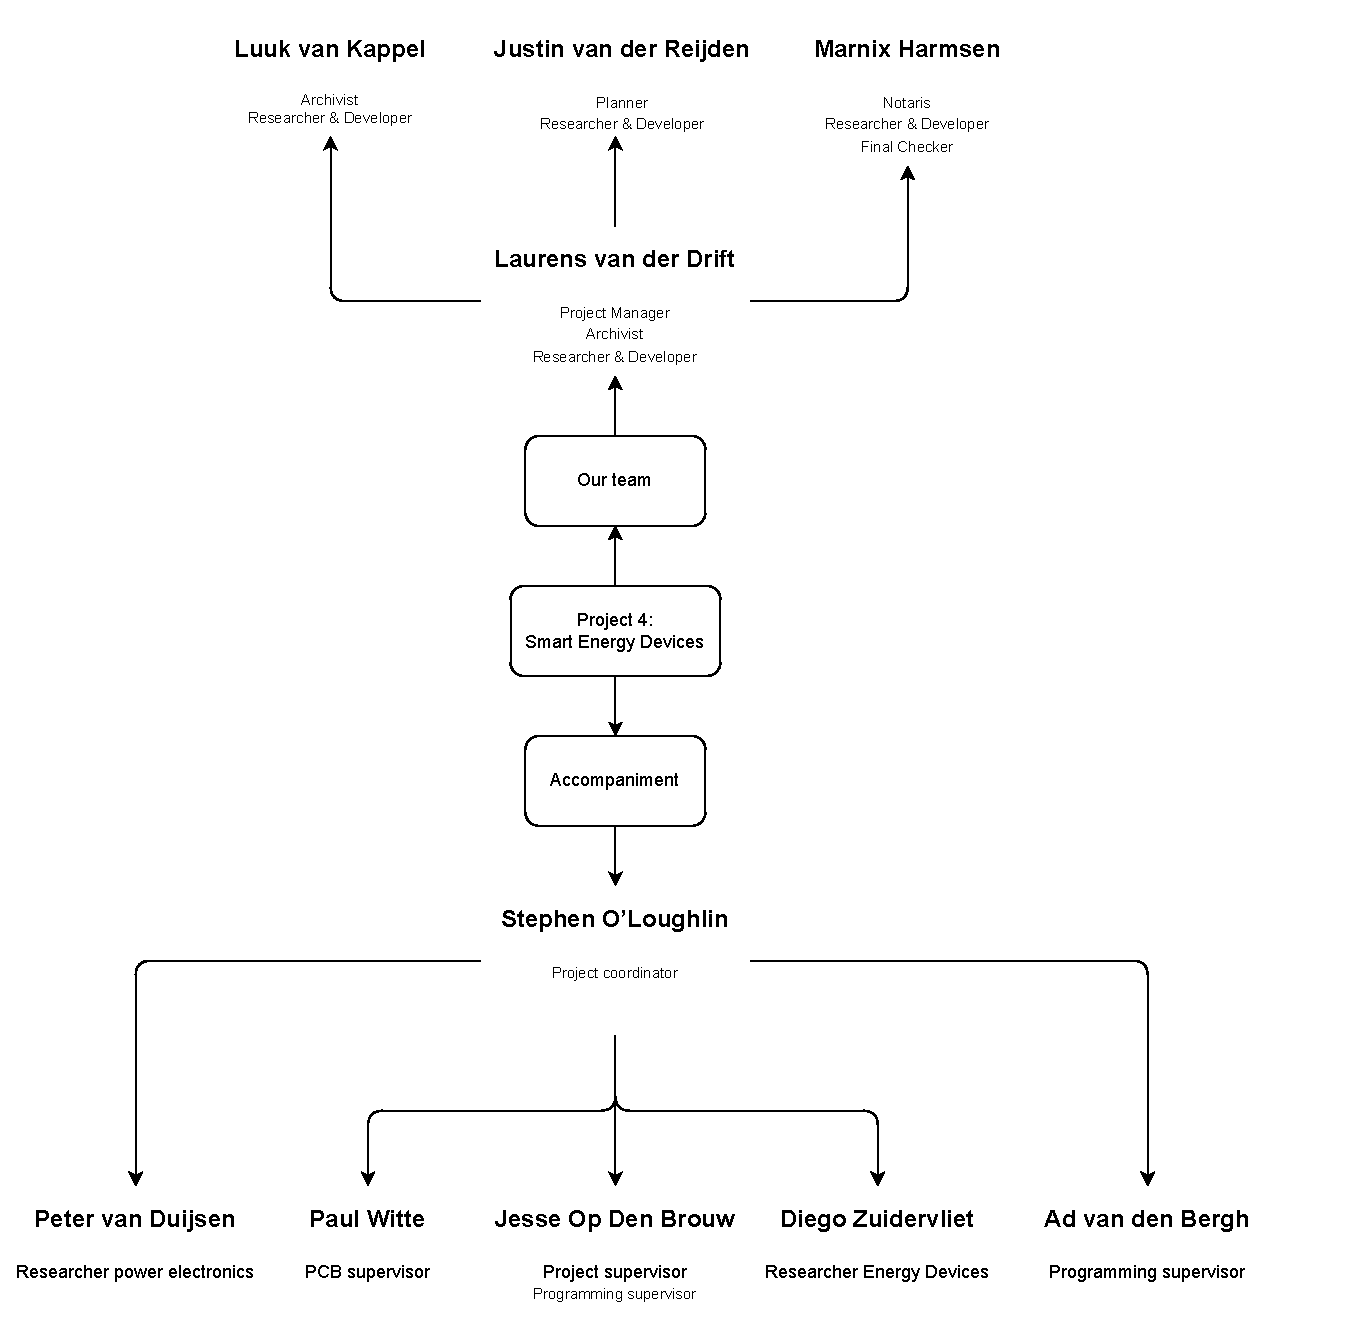
\includepdf[scale=0.9, pages=-]{chapters/Organisation/organisation.drawio.pdf}
    \label{fig:organisation diagram}
\end{minipage}